\chapter{PCM Thermodynamics and Transient Modeling}\label{ch:pcm}

\section{Enthalpy Method and Stefan Interpretation}
For a PCM domain embedded in pores, the apparent-enthalpy method is
\begin{equation}\label{eq:enthalpy_def}
H(T)=\int_{T_{ref}}^{T}\rho c_p\,\mathrm{d}T'+\rho L f_l(T).
\end{equation}
The transient equation becomes
\begin{equation}\label{eq:enthalpy_pde}
\frac{\partial H}{\partial t}=\nabla\cdot\left(k\nabla T\right)+\dot{q}_{src}.
\end{equation}
In a sharp-interface Stefan formulation,
\begin{equation}\label{eq:stefan}
\rho L v_n = k_s\left(\nabla T\cdot\mathbf{n}\right)_s-k_l\left(\nabla T\cdot\mathbf{n}\right)_l.
\end{equation}

\section{Latent Heat and Thermal Buffering}
Liquid fraction is modeled by a smoothed relation:
\begin{equation}\label{eq:liquid_fraction}
f_l(T)=\begin{cases}
0, & T<T_m-\Delta T_m/2,\\
\dfrac{T-(T_m-\Delta T_m/2)}{\Delta T_m}, & |T-T_m|\le\Delta T_m/2,\\
1, & T>T_m+\Delta T_m/2.
\end{cases}
\end{equation}
Thermal buffering efficiency is defined as
\begin{equation}\label{eq:buffering}
\Psi=1-\frac{\max(T_{int})-\min(T_{int})}{\max(T_{src})-\min(T_{src})}.
\end{equation}

\section{Cycle Stability and Degradation Metrics}
Latent heat retention after $N$ cycles:
\begin{equation}\label{eq:latent_retention}
\Lambda_N=\frac{L_N}{L_0}.
\end{equation}
Thermal hysteresis width:
\begin{equation}\label{eq:hysteresis}
\Delta T_{hys}=T_{m,heat}-T_{m,cool}.
\end{equation}

\begin{figure}[htbp]
\centering
\begin{tikzpicture}
\begin{axis}[width=11cm,height=6cm,xlabel={$T$},ylabel={$f_l$},xmin=20,xmax=80,ymin=0,ymax=1.05]
\addplot+[thick] coordinates {(20,0)(40,0)(45,0.25)(50,0.5)(55,0.75)(60,1)(80,1)};
\end{axis}
\end{tikzpicture}
\caption{Smoothed liquid fraction curve used for enthalpy-based PCM simulation.}
\label{fig:pcm_liquid_fraction}
\end{figure}

\begin{figure}[htbp]
\centering
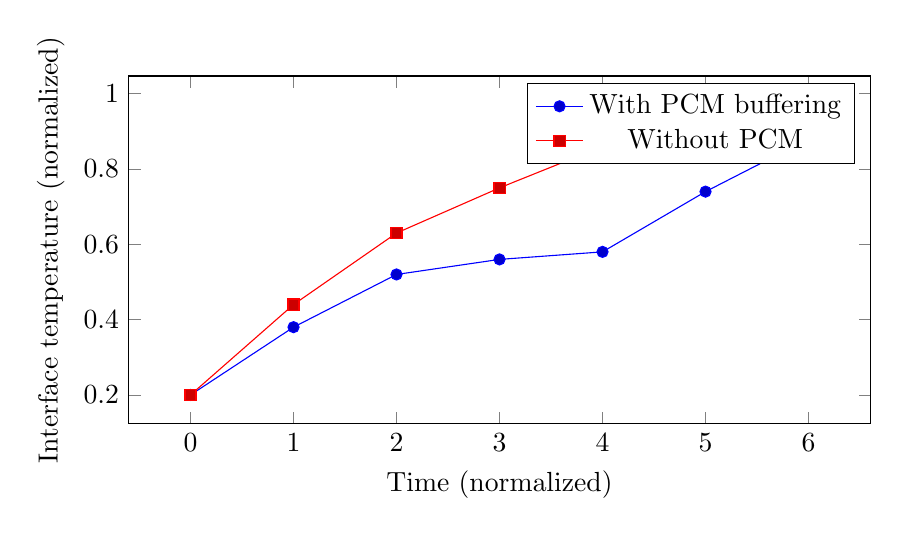
\begin{tikzpicture}
\begin{axis}[width=11cm,height=6cm,xlabel={Time (normalized)},ylabel={Interface temperature (normalized)}]
\addplot+[mark=*] coordinates {(0,0.2)(1,0.38)(2,0.52)(3,0.56)(4,0.58)(5,0.74)(6,0.88)};
\addplot+[mark=square*] coordinates {(0,0.2)(1,0.44)(2,0.63)(3,0.75)(4,0.86)(5,0.93)(6,0.97)};
\legend{With PCM buffering,Without PCM}
\end{axis}
\end{tikzpicture}
\caption{Temperature smoothing induced by latent storage.}
\label{fig:pcm_buffering_curve}
\end{figure}

\begin{table}[htbp]
\centering
\caption{PCM model parameters used in case studies.}
\label{tab:pcm_params}
\begin{tabular}{lcc}
\toprule
Parameter & Symbol & Typical value \\
\midrule
Melting point & $T_m$ & \SI{323}{\kelvin} \\
Latent heat & $L$ & \SI{180}{\kilo\joule\per\kilogram} \\
Solid conductivity & $k_s$ & \SI{0.22}{\watt\per\meter\per\kelvin} \\
Liquid conductivity & $k_l$ & \SI{0.18}{\watt\per\meter\per\kelvin} \\
\bottomrule
\end{tabular}
\end{table}

\begin{table}[htbp]
\centering
\caption{Cycle-stability indicators for embedded PCM (synthetic illustration).}
\label{tab:pcm_cycles}
\begin{tabular}{cccc}
\toprule
Cycles & $\Lambda_N$ & $\Delta T_{hys}$ (K) & Leakage ratio (\%) \\
\midrule
100 & 0.99 & 0.8 & 0.1 \\
500 & 0.97 & 1.0 & 0.3 \\
1000 & 0.95 & 1.2 & 0.6 \\
\bottomrule
\end{tabular}
\end{table}
